\note{This assignment is dedicated to retinal image processing. It should illustrate different parts of the image processing tools, for 
example: filtering, segmentation and some geometrical analysis. Groups of 2 (maximum) are allowed.
Deadline will be fixed in class. Send your through over the campus website. Do not forget your names.}

\section{Introduction}
\begin{wrapfigure}{r}{5cm}
 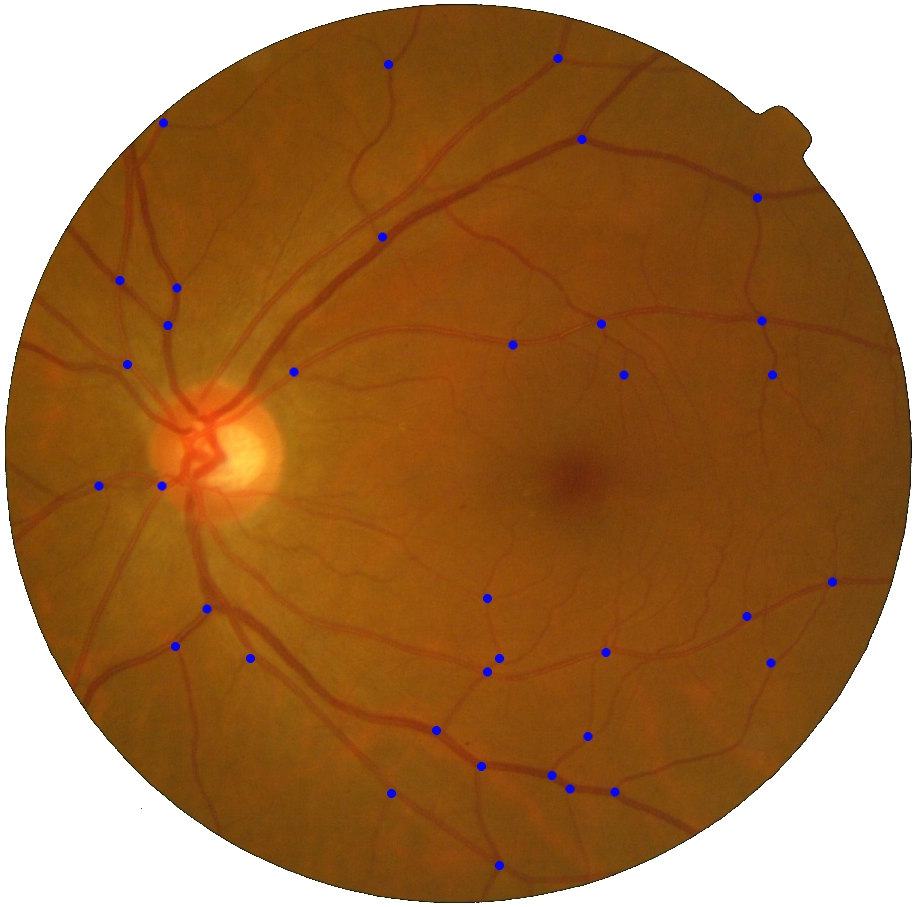
\includegraphics[width=5cm]{im1_points}
\end{wrapfigure}
Ophthalmologists need to observe the retina to detect diseases (like diabete). A wide field observation
of the retina is sometimes necessary, but needs a registration process of several images (in order to create a panoramic 
image). The first step for this process is to detect the T-junctions (bifurcations) of the vessels.

\section{Objectives}

Your objective is to 

\begin{itemize}
\item write a report to explain your method. Please cite your sources and references.
 \item code one or several \matlabregistered{} functions to detect these T-junctions. 
\end{itemize}


At least one of the functions should have this prototype:
\begin{matlab}
function T = t_junctions(retinal_image)
% retinal_image: color (RGB) image of the retina
% T            : binary image representing the T-junctions (points)
\end{matlab}
You are free to develop a method of your own or to look for scientific publications.
Cite the references. An anti-plagiarism software will be employed.
